%\section{Experiment}\label{exp}


%講解實驗規劃與如何呈現數據
\section{實驗目的}
	
	為了改善室內定位的覆蓋率以及定位的精準度,我們利用建置虛擬相片的方法來增加照片的範圍及廣度。有了更多的取樣範圍,藉
由實驗來跟以前傳統的 SIFT 方法做比較。我們分成兩個實驗環境來說明方法所改善的定位數據:(1)可以控制的實驗環境、(2)一般
室內定位的環境。

	首先製造一個可以控制特徵點數量的環境,在這個環境中我們驗證每個固定距離內根據 SIFT 所涵蓋的特徵點數量作比較,增加
與物體的固定距離算出每個距離中的平均定位誤差,再算出定位誤差範圍的覆蓋率與傳統的照片影像定位作比較。在可以控制的定位環
境下我們根據這些實驗方法說明改善的成果,再把方法放建築一般實際的室內環境中作比較,最後呈現出改善的平均定位誤差與增加環
境所能定位的覆蓋率。為了完成這些實驗,所用到的設備為  Intel Core I5 2.0GHz 的CPU與 8 GB 的RAM,顯卡為了能夠使
用 CUDA 平行運算加速,所採用的是 Nvidia 的顯示晶片。

%1. Controlled Enviornment 
\section{可控制環境定位數據比較}


% 控制環境實驗目的與成效描述
\subsection{可控制環境實驗方法}
	建立可以控制的實驗環境主要目的為在可以控制的特徵點環境下與一般平面影像定位做比較,藉由實驗驗證出有更好的定位覆蓋率
與更小的平均定位誤差。在根據有限景物數量的環境下,將待定位的照片依距離增加,生成出格狀的位置的照片定位點,每個定位點前後
都有固定的間距距離,利用這些待定位照片,分別用三種方法比較實驗結果。

	一開始建置實驗環境,我們將這些定位照片分布在 4公尺 X 5公尺的環境大小內,而景物的分布在 1.5公尺 X 0.7公尺的大小範圍內, 
Kinect 攝影機放置在距離景物 0.5公尺前的地方,利用 Kinect 攝影機拍照取得深度照片與待定位的照片。如圖\ref{table:Controlled 
EV parameters}所示,在兩個控制環境的實驗中,利用不同的定位環境、不同的間距以及不同待定位圖片的數量來做實驗比較。
		
		
%放圖顯示Uniform 	Permutation 與 Random Permutation
		
\begin{table}[htbp]
  \centering
  \caption{控制環境實驗參數設定}
    \begin{tabular}{rrr}
    \toprule
    實驗設定 :  & 控制環境 1 & 控制環境 2 \\
    \midrule
    待定位照片數量 : & 45 張  & 54 張 \\
    間距寬度 : & 0.5m & 0.5m \\
    間距長度 : & 0.75m & 0.5m \\
    \bottomrule
    \end{tabular}%
  \label{table:Controlled EV parameters}%
\end{table}%


\subsection{可控制環境實驗數據分析}

	為了證明在可以控制的環境下有比較好的定位結果,將實驗分成三個部分做討論:
	
\begin{itemize}
  \item (1) 特徵點數量分布分析
  \item (2) 間距定位誤差分布分析
  \item (3) 定位精準度覆蓋率以及平均定位誤差
\end{itemize}
		
\subsubsection{特徵點數量分布分析}

	這個實驗目的是要看出根據景物的距離增加與特徵點數量的關係圖,實驗的作法是先在待定位圖片的第一排中間設為圓心,如圖
\ref{fig:CoverDisk}所示。根據這個圓心將圓的半徑以 0.5公尺的長度增加,依據每個圓之間所能覆蓋的特徵點位置做特徵點數量的總和並算
出平均值,藉由圖中的趨勢看出特徵點數量的變化。

\begin{figure}
\begin{center}
  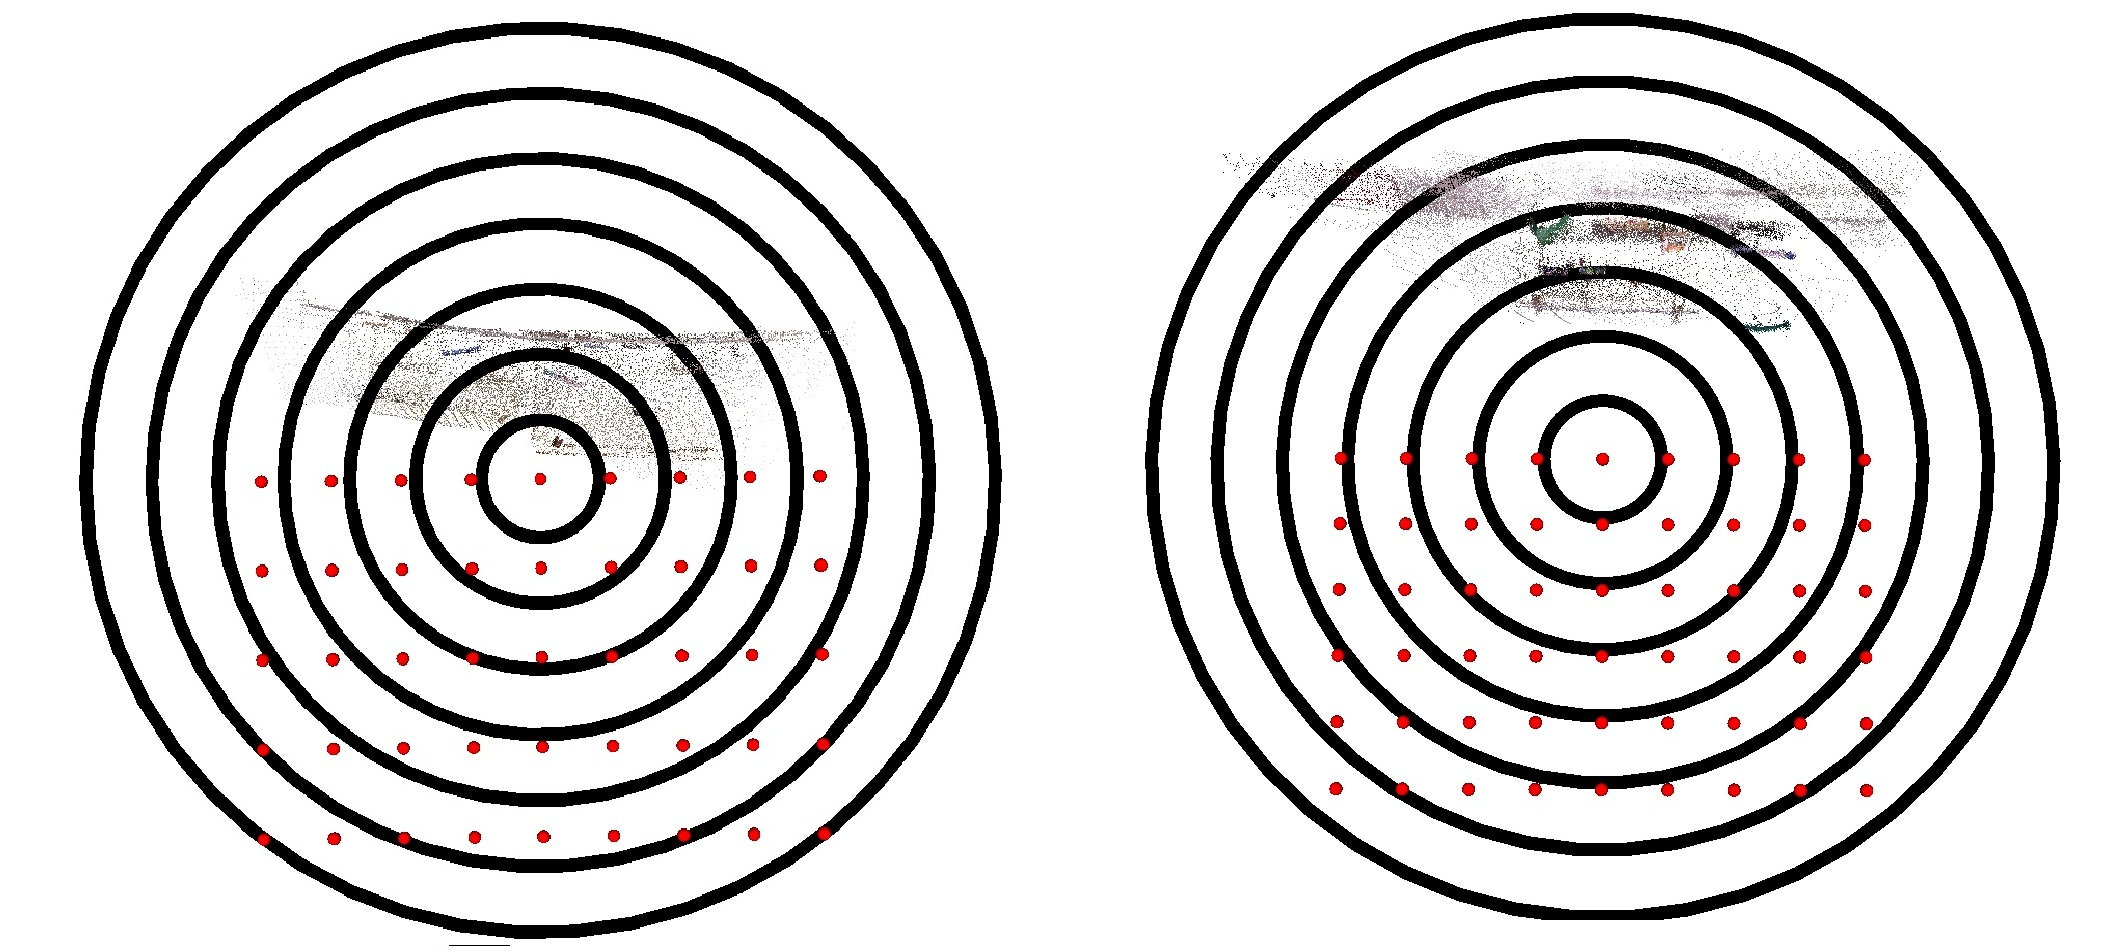
\includegraphics[width=1.0\textwidth]{figures/CoverDisk.jpg}
  \caption{依照同心圓的覆蓋算出每個半徑內的每張圖的特徵點平均數,左.控制環境 1 右.控制環境 2}
  \label{fig:CoverDisk}
\end{center}
\end{figure}
	
	如圖\ref{fig:CoverDisk_DescriptorNum}所示,橫軸表示與景物之間的距離增加,縱軸為特徵點的數量,三條線分別代表 1.2D隨機排列
的攝影機影像位置,2.3D隨機排列的虛擬攝影機影像位置與 3.3D格狀排列的虛擬攝影機影像位置,一開始距離越近根據2D影像所找出的影像特徵點也
越多,符合實際的情況,但之後的趨勢分布呈現卻發現距離越遠平面影像所找出的特徵點減少許多,表示說2D平面影像因為受到攝影機位置取樣的關係都
侷限在景物附近,導致距離越遠卻沒有好的匹配影像做比對,但是3D虛擬影像的好處在於可以分布在整個環境區域中模擬平面影像所照出的照片,所以特
徵點的數量不會因距離增加而有太大的改變,對於之後的定位精準度也不會因為距離增加而導致定位誤差有明顯擴大的影響。
			
\begin{figure}
	\begin{center}
    \subfigure[控制環境 1.特徵點平均數量比較]{\label{fig:CoverDisk_Descriptor1}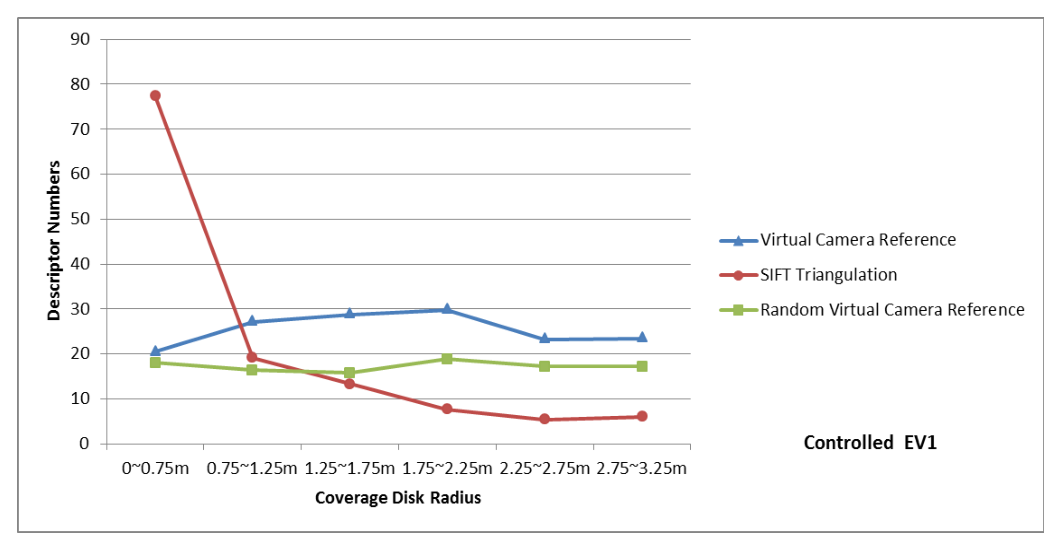
\includegraphics[width=0.45\columnwidth]{figures/Controlled_EV1_DescriptorNum.eps}}
    \subfigure[控制環境 2.特徵點平均數量比較]{\label{fig:CoverDisk_Descriptor2}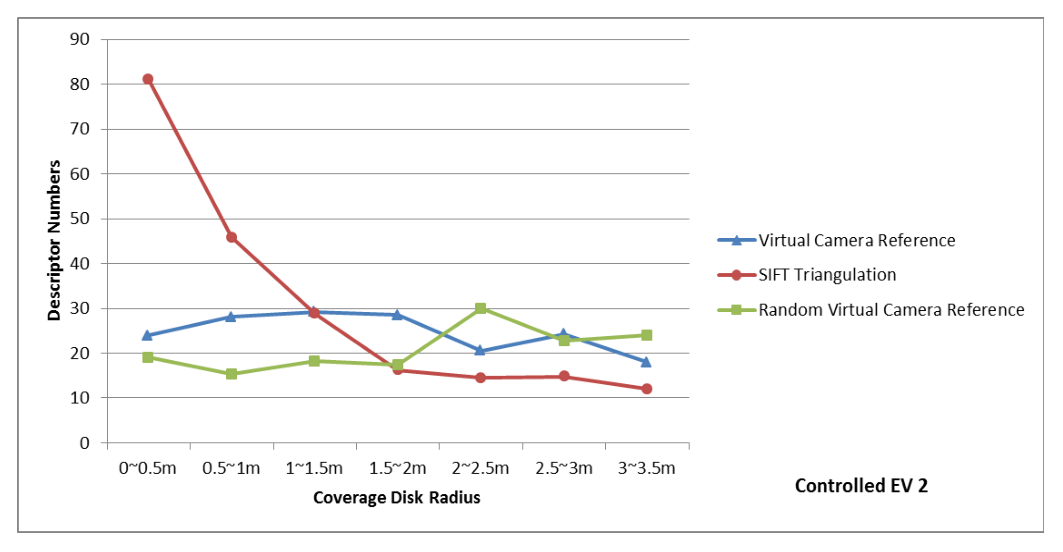
\includegraphics[width=0.45\columnwidth]{figures/Controlled_EV2_DescriptorNum.eps}}
	\end{center}
  \caption{特徵點數量趨勢圖}
  \label{fig:CoverDisk_DescriptorNum}	
\end{figure}
	
\begin{figure}
	\begin{center}
    \subfigure[控制環境 1.間距定位平均誤差比較]{\label{fig:Distance_Error1}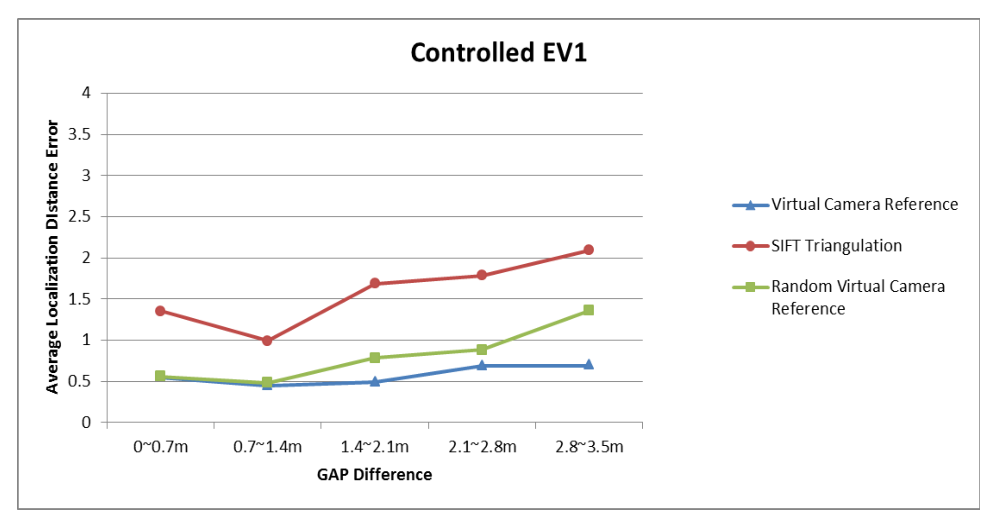
\includegraphics[width=0.45\columnwidth]{figures/Controlled_EV1_Localization_Distance_Error.eps}}
    \subfigure[控制環境 2.間距定位平均誤差比較]{\label{fig:Distance_Error2}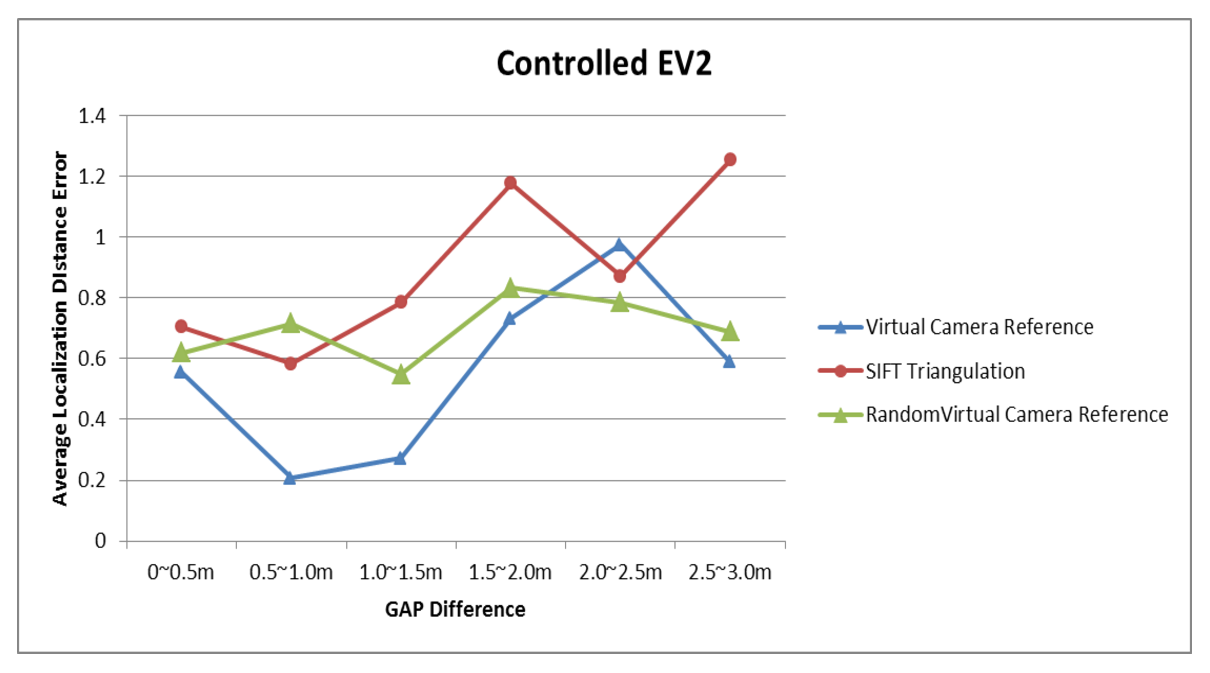
\includegraphics[width=0.45\columnwidth]{figures/Controlled_EV2_Localization_Distance_Error.eps}}
	\end{center}
  \caption{間距定位平均誤差趨勢圖}
  \label{fig:Localization_Distance_Error}	
\end{figure}	
	
\subsubsection{間距定位誤差分布分析}	
	
	以圖\ref{fig:Localization_Distance_Error}可看出,以每一橫排的待定位圖片的平均誤差分布,根據每一個不同的間距,虛擬相機圖片定位比一般相機所做出的影像定位誤差都有改善,
尤其以格狀分布的3D虛擬影像改善最為明顯。根據我們的方法,我們想要模擬在不同的角度及位置產生3D虛擬影像,比起一般的傳統影像有更多可以
做特徵點匹配的相片可供使用。傳統的平面影像定位所做出的資料庫中,對於景物比較遠的照片並沒有資訊提供,只能利用拘限在景物較近的照片可供定位,
但是少許的特徵點使得定位誤差更加放大,所以照圖中趨勢來看,距離一增加,定位誤差就會加大。但是在3D虛擬影像不會因為距離的增加,導致定位
誤差增加。除了3D虛擬影像可以增加更多可以被匹配的相片以外,好的虛擬相機分布,也可以產生更多的特徵點可以被匹配。以隨機分布與格狀分布來說
,隨機分布的3D虛擬相片雖然有改善,但沒有比格狀分布的虛擬相片改善來的明顯。在我們的方法中,我們定位會參考照相機所在的位置,所以定位的位置
都會在相機位置的附近,隨機分布可能會造成某些區域的相機分布過於集中,某些相機卻又過於分散的情況發生。所以在隨機虛擬相機分布的定位其實就跟
平面相機分布的定位分布差不多,差別在於相片角度會避開障礙物,但不會均勻分布在環境中;格狀平均分布的攝影機位置,就會均於分布在環境內,而對
於影像特徵點匹配上比隨機分布來的更有幫助。


\subsubsection{定位精準度覆蓋率以及平均定位誤差}	

	當發現與景物的距離越遠在3D虛擬影像定位並不會影響誤差,整體來看,對定位的覆蓋率也有一定的提升。根據圖所示,在(控制環境1裡的圖)說明均
勻分布的3D虛擬相機定位在誤差0.5公尺左右有超過$60\%$的覆蓋率,但隨機分布的虛擬相機以及2D平面影像定位坐落在$20\%$左右上下,表示相機的分
布影響定位結果的好壞。這也是我們想讓照相機分布平均的原因,再回到圖\ref{fig:CoverDisk_Descriptor1}來看,在1.75公尺以後的隨機虛擬相
片所找出特徵點平均數量比起格狀分布虛擬相片所找出的特徵點數量少上許多,而在圖\ref{fig:Distance_Error1}來看,每個間距的定位平均誤差,
格狀分布都比隨機分布的誤差好上許多。所以當以誤差在0.6公尺以內的覆蓋率來說,隨機分布的虛擬相片並沒有產生比較好的定位覆蓋率,但以格狀分布的
虛擬相片定位覆蓋率與2D影像定位覆蓋率相比,結果好上許多。平均定位的誤差以格狀的虛擬影像為物誤差為最低,2D影像定位的誤差為最高,改善了整體定
位的平均誤差。


%2. Indoor Localization
\section{一般室內環境定位數據比較}

	在控制環境下,改善了定位的覆蓋率與精準度,在這章節我們將測試在一般室內環境下的定位測試。我們將室內定位環境分成三種情境:(1)
居家客廳 ,(2) 居家廚房與 (3)居家房間,分別在這三種環境下進行定位實驗。在一般室內定位主要進行定位覆蓋率與定位平均誤差測試。
	
\subsection{一般室內定位環境實驗方法}
	
	在室內定位的情況下,拍攝待定位照片的方法依據環境情況而定。待定位照片拍攝方法是依照人能夠活動的範圍作依據,在這些區域進行
格點分布拍攝,如圖所示。每張待定位圖片的間距距離為0.5公尺,照片數量根據環境大小而定,平均在20張上下。虛擬照片依據間距距離,取出
不同數量的虛擬相機。因為考量不同環境的景物分布,每組相機位置分別拍攝兩種不同的角度,最後根據虛擬相機拍攝出的照片作影像定位。除了
與2D影像定位方法做比較之外,分別測試在不同虛擬照片資料數量的定位情形。在圖中,是客廳的點雲環境,如同之前實驗利用點雲環境拍攝虛擬
照片,圖為定位平均誤差分布的情形
	
